% SVN info for this file
\svnidlong
{$HeadURL$}
{$LastChangedDate$}
{$LastChangedRevision$}
{$LastChangedBy$}

%\chapter{Why is Testing and Supporting Documentation Important?}
%\chapter{Why is Testing driven by Supporting Documentation Important?}
\chapter{Document-Driven Testing for Optimal Deployments}
%\chapter{HIL and BMI Ecosystem}
\labelChapter{Chapter_1}

\begin{introduction}
  %This chapter will describe from the ground up the theory of types and how to evolve them.
  \begin{flushright}
  \vspace{-13mm}The fundamental principle of science, the definition almost, is this: \\ the sole test of the validity of any idea is experiment. \\
  --- Richard P. Feynman
  \end{flushright}
\end{introduction}


\text{}\vspace{-18mm}
\section{How to guarantee a defect-free software product}

\lettrine[nindent=-1pt]{A}{software product can be deemed defect-free} if all the requirements have been completely covered by tests supporting the specifications, and are continuously validated throughout the development cycle.  A development team always strives to provide such guarantees, which can be achieved by being \emph{diligent} in following specific software development practices and ensuring that the requirements are bounded and reflected through \index{complete coverage}\emph{complete coverage}.  \\


One methodology of ensuring that such a continuity is preserved, is via the \index{V-Model}V-Model of software development\footnote{\link{http://ccdocs.berkeley.edu/content/system-validation-plan}} illustrated in Figure \ref{fig:v-model}.

%\image{0.16}{figures/BMIFLOW.png}{HIL and BMI Ecosystem. \emph{Special thanks to Gerardo for providing this figure.} }

\begin{figure}[!h] % Example of including images
\begin{center}
%\includegraphics[width=0.5\linewidth]{#1}
%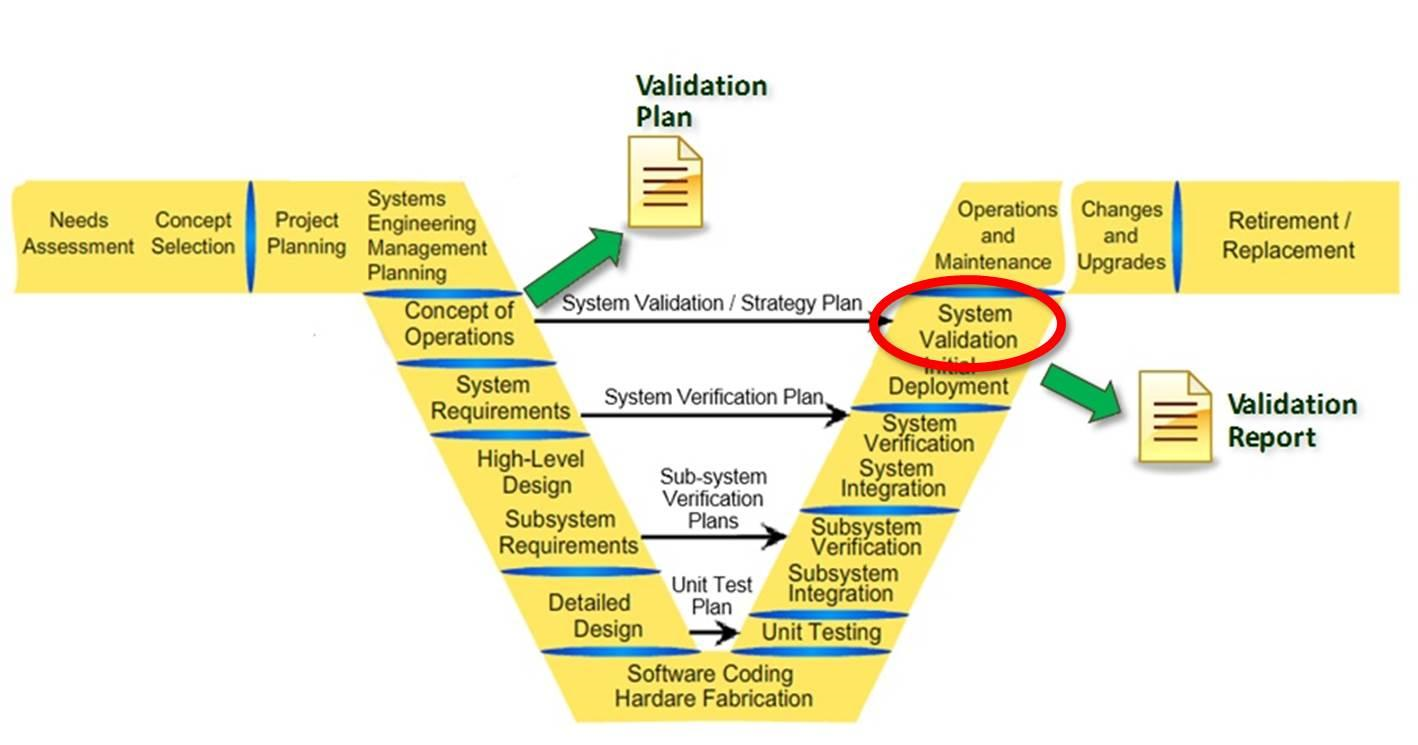
\includegraphics[scale=0.36]{figures/v_diagram_-_validation_plan2.png}
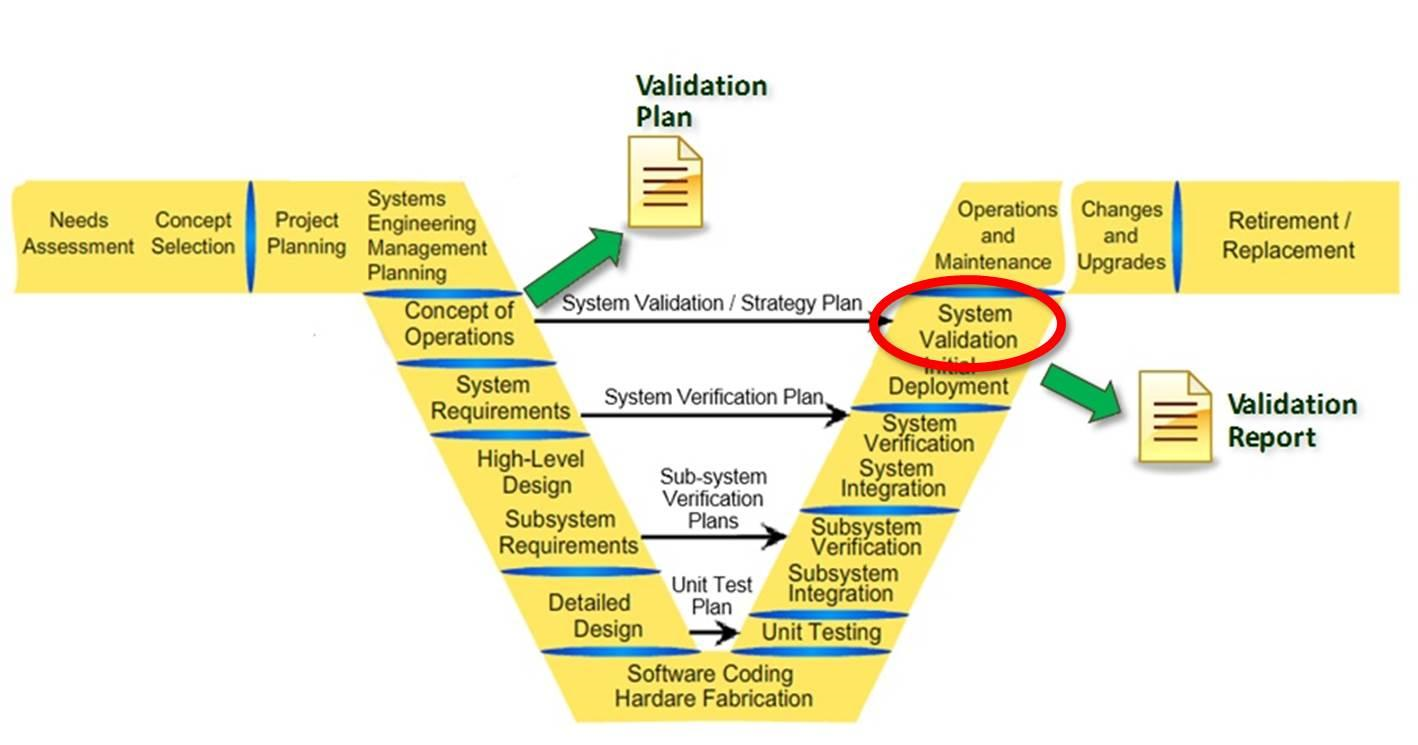
\includegraphics[scale=0.52]{figures/v_diagram_-_validation_plan2.png}
\end{center}
\caption{The V-Model of software development}
\label{fig:v-model}
\end{figure}

\pagebreak

If you bisect vertically the V-Model, you will notice that \underline{each requirement} -- or implementation -- on the left-hand side is \emph{supported} by a verification or validation step on the right-hand side.  This ensures that the scope is bounded and provides complete coverage\footnote{Coverage ensures all aspects of the codebase are verified and asserted via test(s).}.  For every step \underline{documentation is critical} to both \emph{specify} the requirements, and then to subsequently \emph{validate} against those requirements.

%all the steps throughout the development .  Types might at times seem burdensome, but if viewed correctly can provide insight in how to naturally create or evolve the construction of APIs. \\

%Below is 

\section{Testing Under Changing Environments Via System Testing}

There will be times where \emph{Integration Testing} is not enough.  This is where \index{system testing}\emph{System Testing}\footnote{Ashfaque Ahmed and Bhanu Prasad. 2016. \emph{Foundations of Software Engineering.} Auerbach Publications, Boston, MA, USA.} comes in.  Here we take the software product as a \emph{black box} --  as opposed to in Integration Testing -- and test it under different environments without touching the code-base.  One of the best ways to ensure that the software product will operate as defined by the \emph{requirements} is to run \emph{end-to-end scenarios} with validation.  This requires one to have a list of \emph{functional specifications} that the software product must perform, and to create one or more workflows where these will be pipelined together to generate this type of \index{functional testing}\emph{Functional Testing}\footnote{Functional Testing validates the software design based on the requirement specifications, by running tests to check that the software's features match the functional specifications.}.  \\

For BMI these are defined as follows: \\

\begin{itemize}
\item[\code{pro }$\blacktriangleright$\hspace{-12mm}] \hspace{10mm}\emph{Provisions a node.}
\item[\code{dpro }$\blacktriangleright$\hspace{-12mm}] \hspace{10mm}\emph{Deprovisions a node.}
\item[\code{snap }$\blacktriangleright$\hspace{-12mm}] \hspace{10mm}\emph{Takes a snapshot of a node.}
\item[\code{ls }$\blacktriangleright$\hspace{-12mm}] \hspace{10mm}\emph{Lists store images.}
\item[\code{import }$\blacktriangleright$\hspace{-12mm}] \hspace{10mm}\emph{Importing images or snapshots into BMI for provisioining.}
\item[\code{db }$\blacktriangleright$\hspace{-12mm}] \hspace{10mm}\emph{Database commands that about imported images or snapshots.} \\
\end{itemize}

By then integrating these into an end-to-end workflow, one can perform all these and ensure that the basic requirements are satisfied.  An example of a possible end-to-end workflow is described in Figure \ref{fig:end_to_end_workflow}. %as follows:

\begin{figure}[!h] % Example of including images
\vspace{10mm}
\label{fig:bmi-workflow-end-to-end}
\begin{center}
%\includegraphics[width=0.5\linewidth]{#1}
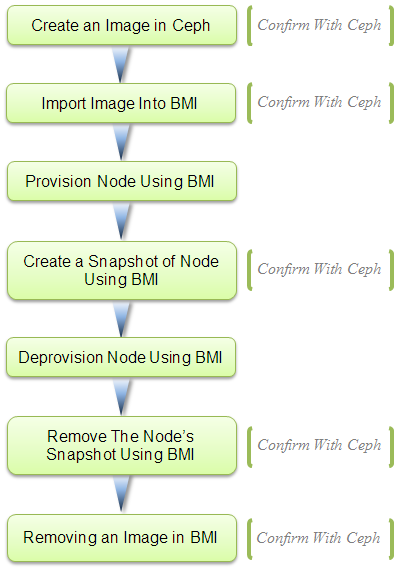
\includegraphics[scale=0.7]{figures/bmi-workflow-with-image-cleanup-v2.png}
\end{center}
\caption{An example of an end-to-end workflow}
\label{fig:end_to_end_workflow}
\end{figure}

%\section{Building a System Testing Framework via The Scientific Method}
\section{Behavior-Driven Development: A Scientific-Method Approach to Testing}

The \index{scientific method}\emph{Scientific Method} is an unbiased approach to discovering what the facts truly about a system by progressing using \emph{systematic doubt}\footnote{Morris Raphael Cohen and Ernest Nagel. 1934. \emph{An Introduction to Logic And Scientific Method.} Harcourt, Brace and World, New York, NY, USA.} to ensure adequate evidence support each problem being solved.  The facts are not gathered unless there is a problem being defined upon which relevant facts are required to prove or disprove inquiries (\emph{hypotheses}) about the problem. \\




\index{Behavior-Driven Development (BDD)}Behavior-Driven Development (BDD) is defined through a live document implemented using the Gherkin language\footnote{\link{https://github.com/cucumber/cucumber/wiki/Gherkin}}, which utilizes \emph{Given-When-Then} control-flow syntax defined as follows: \\

\begin{itemize}
\item[\index{BDD (Given)}\code{Given }$\blacktriangleright$\hspace{-12mm}] \hspace{10mm}\emph{Defines a given state.}
\item[\index{BDD (When)}\code{When }$\blacktriangleright$\hspace{-12mm}] \hspace{10mm}\emph{Defines a given action performed under the given state.}
\item[\index{BDD (Then)}\code{Then }$\blacktriangleright$\hspace{-12mm}] \hspace{10mm}\emph{Defines the expected outcome after the action is performed.} \\
\end{itemize}

By building a \emph{scenario} through combining these into premises using the \emph{Given}- and \emph{When}-initiated statements, we are able to discover if our system is validated at each step and confirm the \emph{Then} conclusion statement(s).  Thus we are hypothesis-driven through a BDD-model of our system to ensure it matches our expected \emph{operational semantics}\footnote{\link{https://en.wikipedia.org/wiki/Operational_semantics}}. \\

%\pagebreak

An example of such an end-to-end scenario for BMI is illustrated in Figure \ref{fig:chp1_bdd-bmi-end-to-end-template}, where each line is a step that references an implemented function. \\

The \index{end-to-end scenario}end-to-end scenario is a \emph{model} used as a set of \emph{rules of inference} guided by an ordered collection of \index{premises}\emph{premises} -- which are assumed to be \emph{true} -- and \index{conclusions}conclude that \emph{all} the steps are \emph{truth preserving}:

\begin{center}
$$Premises \implies Conclusions$$
\end{center}

\pagebreak

\begin{figure}[!h] % Example of including images
%\label{fig:ceph-imported-cloned-image}
\begin{center}
%\includegraphics[width=0.5\linewidth]{#1}
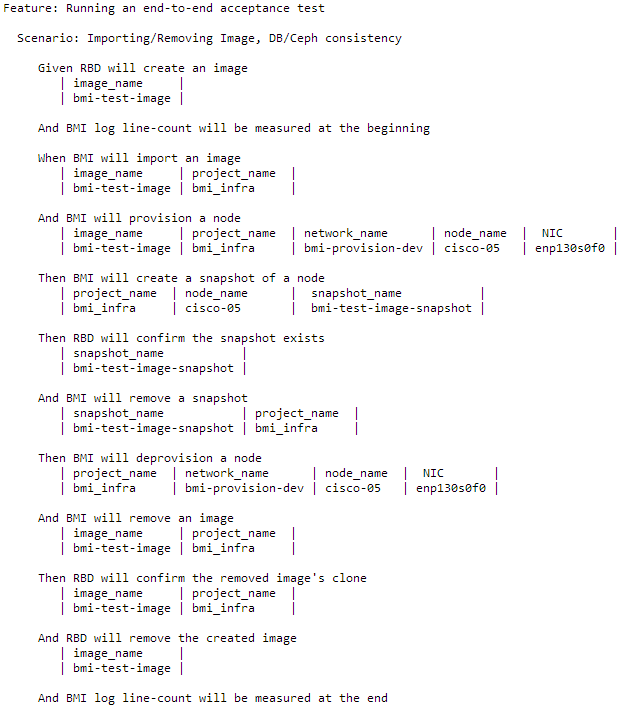
\includegraphics[scale=1]{figures/end-to-end-bdd-template.png}
\end{center}
\caption{The BMI End-to-End Behavior-Driven Deployment Test, with tables of parameters to test with}
%\label{fig:example_figure}
\label{fig:chp1_bdd-bmi-end-to-end-template}
\end{figure}





For example, in Figure \ref{fig:chp1_bdd-bmi-function-definition} the creation of a RADOS block device (RBD\footnote{Ceph Storage provides the ability for its (bootable) images to be mountable remotely using a RADOS block device.  For more information please proceed to the following web location: \\  \link{https://docs.openstack.org/mitaka/config-reference/block-storage/drivers/ceph-rbd-volume-driver.html}}) mountable image at the start is defined through the \code{rbd\_create\_image()} function, where it is decorated by the sentence referenced in the live-document. \\

\text{}\vspace{10mm}

\pagebreak

%
\begin{figure}[!h] % Example of including images
%\label{fig:ceph-imported-cloned-image}
\begin{center}
%\includegraphics[width=0.5\linewidth]{#1}
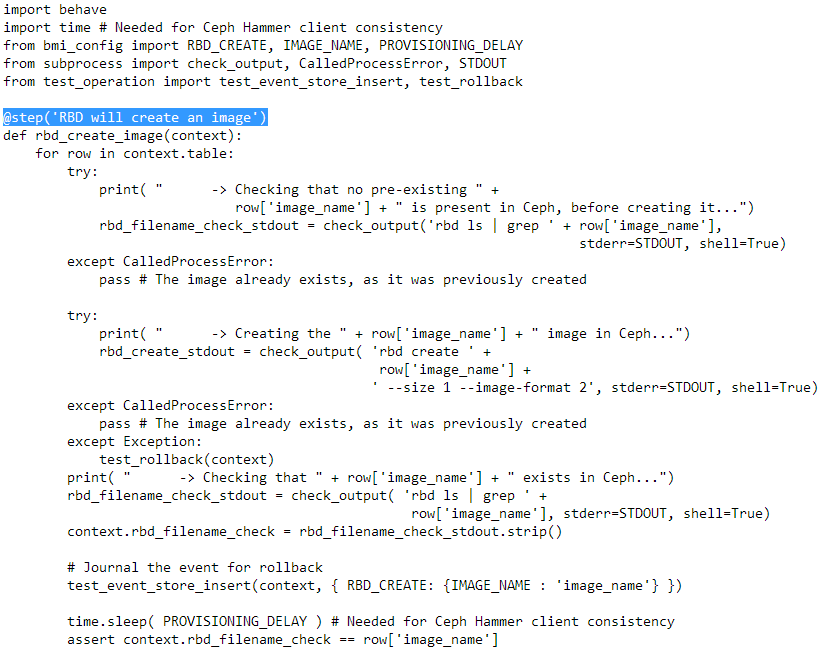
\includegraphics[scale=1]{figures/bmi-bdd-step-definition-v3.png}
\end{center}
\caption{The definition of the RBD creation step, where the decoration highlights the sentence referenced in the end-to-end deployment test}
%\label{fig:example_figure}
\label{fig:chp1_bdd-bmi-function-definition}
\end{figure}

\text{}\vspace{10mm}

In the next chapter, you will learn how to configure and run an acceptance test.